\documentclass{article}

% NeurIPS 2026 workshop, double-blind reviewing.
\usepackage[dblblindworkshop]{neurips_2026}

\usepackage[utf8]{inputenc}
\usepackage[T1]{fontenc}
\usepackage{hyperref}
\usepackage{url}
\usepackage{booktabs}
\usepackage{amsfonts}
\usepackage{amsmath}
\usepackage{nicefrac}
\usepackage{microtype}
\usepackage{xcolor}
\usepackage{graphicx}
\usepackage{float}
\hypersetup{hidelinks,hypertexnames=false}

\title{Mixing Matters: Evidence Position Bias Across Attention and
State-Space Language Models}

\workshoptitle{New in ML}

\author{Anonymous Author(s)}

\begin{document}

\maketitle

\begin{abstract}
Language models often answer multi-document questions less accurately when the relevant document appears in the middle of the context.
We ask whether the sequence mixer changes this accuracy-versus-position curve under approximately matched pretraining data, scale, and context.
Our deterministic evaluation moves one gold document through ten positions while holding the question and nine distractors fixed.
We summarize start and end advantages with primacy and recency edges and use a question-level paired bootstrap with 10{,}000 resamples and Holm correction.
On 800 exploratory questions, Pythia-2.8B has a positive primacy edge ($+0.052$, 95\% CI $[0.032,0.072]$), while two Pile-trained Mamba variants do not ($-0.001$ and $-0.018$); both paired architecture interactions exclude zero.
A more tightly matched 8B Mamba-2 pair is directionally consistent: the hybrid containing 7\% attention layers has a larger primacy edge than the pure model, but the paired difference is uncertain ($+0.019$, 95\% CI $[-0.006,0.044]$, Holm $p=0.144$).
Scale, corpus, synthetic retrieval, prompt, attention-sink, and linear-probe analyses further bound the result.
Together they establish an exploratory architecture-position interaction and motivate, but do not yet prove, an attention-based mechanism.
\end{abstract}

\section{Introduction}
\label{sec:intro}

Transformers often read multi-document contexts unevenly: accuracy peaks when the answer-bearing document is near an edge and falls in the middle \citep{liu2024lost}.
This behavior matters because retrieval systems cannot assume that all evidence positions are equally usable.
Prior work links lost-in-the-middle behavior to U-shaped attention patterns \citep{hsieh2024found}, but model-family comparisons still confound sequence mixing with data, tokenizer, scale, depth, and positional encoding.
State-space models such as Mamba \citep{gu2023mamba,dao2024mamba2} provide a useful contrast because they compress the prefix into a recurrent state instead of using dense causal attention.

We make three contributions.
First, we build an auditable ten-position evaluation with floor and ceiling anchors, preserved generations, and inference settings recorded per example.
Second, we find a paired architecture-position interaction in a Pile-trained 2.8B comparison and test it with a more tightly matched 8B pure/hybrid pair.
Third, we organize scale, corpus, task, prompt, sink, and probe results into mechanistic evidence with explicit uncertainty.
All reported results use an exploratory split; the held-out confirmatory split remains unspent.

\section{Related work}
\label{sec:related}

\paragraph{Position bias in long contexts.}
\citet{liu2024lost} established the lost-in-the-middle curve in retrieval and multi-document QA.
Subsequent work measures effective context length \citep{hsieh2024ruler}, associates the curve with attention allocation \citep{hsieh2024found}, and proposes context-use interventions \citep{an2024make,peysakhovich2023attention}.
We focus on whether the curve changes across sequence mixers.

\paragraph{Sequence mixers.}
Dense self-attention \citep{vaswani2017attention} mixes token pairs under a causal mask, while Mamba and Mamba-2 carry information through selective state-space recurrences \citep{gu2023mamba,dao2024mamba2}.
Hybrid models interleave the two mixers \citep{lieber2024jamba,nvidia2025nemotronh}.
\citet{waleffe2024empirical} release the pure and hybrid 8B Mamba-2 checkpoints used in our tightest controlled comparison.

\paragraph{Attention sinks.}
\citet{xiao2024efficient} showed that causal transformers can concentrate attention on initial tokens.
We test whether this attention-sink statistic covaries with primacy, treating the result as correlational because a valid sink-blocking ablation is absent.

\section{Measurement and statistics}
\label{sec:method}

\paragraph{Task and anchors.}
We use the 2{,}655 released questions from the Lost-in-the-Middle 10-document QA setting \citep{liu2024lost}.
Each question has one gold document and nine distractors.
We build ten prompts per question, moving only the gold document through positions $0$ to $9$ while retaining the same distractors and token budget.
A no-gold floor measures guessing or memorized knowledge, and a gold-only ceiling measures answerability under perfect retrieval.

\paragraph{Edges and statistics.}
Let $a_S$, $a_M$, and $a_E$ be mean accuracy at start positions $\{0,1\}$, middle positions $\{4,5\}$, and end positions $\{8,9\}$.
We define primacy as $a_S-a_M$ and recency as $a_E-a_M$.
The question is the unit of analysis.
Each of 10{,}000 bootstrap samples draws complete ten-position question bundles with replacement, and model comparisons reuse the same sampled questions.
We report percentile 95\% confidence intervals and Holm-correct the primacy and recency tests within each comparison family.
The fixed split contains 800 exploratory and 1{,}855 confirmatory questions.
Only the exploratory split is reported.

\paragraph{Reproducibility and controls.}
The harness vendors the official prompt builder and \texttt{best\_subspan\_em} scorer at a pinned commit.
It also records normalized exact match and first-line extraction.
Generation is greedy with temperature $0$, at most 32 new tokens, fixed seeds, BF16 where supported, pinned model revisions, and one Mamba execution path.
Each unique run preserves prompts, raw generations, failures, token counts, software versions, and decoding settings.
The released key-value task provides an executed positive control: the pipeline detects a $+0.38$ Pythia start-versus-middle effect.
Negative and distractor-order controls are implemented but have no committed run artifacts, so we do not count them as passed controls.

\section{Architecture comparisons}
\label{sec:contrast}

\paragraph{Primary 2.8B comparison.}
We compare \texttt{pythia-2.8b} \citep{biderman2023pythia} with \texttt{mamba-2.8b} and \texttt{mamba2-2.7b}.
All are base models pretrained on the Pile \citep{gao2020pile}, have similar parameter counts, and use related tokenizers.
Table~\ref{tab:phase2} and Figure~\ref{fig:phase2} show a positive primacy edge for Pythia and no positive primacy edge for either Mamba model.
The paired Mamba-minus-Pythia primacy interactions are $-0.053$ and $-0.070$ (both Holm $p<10^{-4}$), while Mamba-1 versus Mamba-2 is uncertain ($+0.017$, 95\% CI $[-0.005,0.038]$).
All three models have positive recency edges.
These comparisons match corpus and approximate scale, but not depth, positional encoding, state size, or checkpoint family.

\begin{table}[H]
\caption{Pile-trained models on 800 exploratory questions.
Intervals use a question-level paired bootstrap; $p$ is Holm-corrected.}
\label{tab:phase2}
\centering
\scriptsize
\begin{tabular}{@{}lccc@{}}
\toprule
Model & Primacy (95\% CI) & Recency (95\% CI) & Floor / Ceiling \\
\midrule
\texttt{pythia-2.8b} & $+0.052$ $[0.032,0.072]$, $p{<}10^{-4}$ & $+0.075$ $[0.054,0.097]$, $p{<}10^{-4}$ & $0.091 / 0.640$ \\
\texttt{mamba-2.8b} & $-0.001$ $[-0.016,0.014]$, $p{=}0.91$ & $+0.077$ $[0.058,0.097]$, $p{<}10^{-4}$ & $0.115 / 0.615$ \\
\texttt{mamba2-2.7b} & $-0.018$ $[-0.034,-0.003]$, $p{=}0.02$ & $+0.105$ $[0.086,0.124]$, $p{<}10^{-4}$ & $0.128 / 0.619$ \\
\bottomrule
\end{tabular}
\end{table}

\begin{figure}[H]
\centering
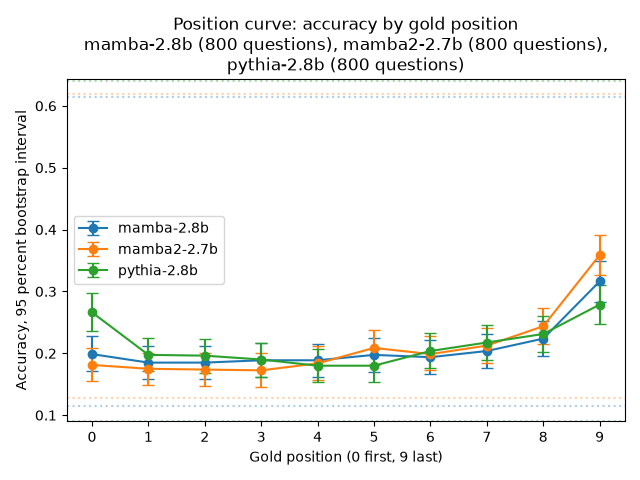
\includegraphics[width=0.52\linewidth]{figures/phase2-curves.png}
\caption{Accuracy versus gold position in the 2.8B comparison.
Pythia rises at the start; all models rise at the end.
Dotted lines are each model's floor and ceiling.}
\label{fig:phase2}
\end{figure}

\paragraph{Matched 8B attention comparison.}
Our strongest control uses NVIDIA's pure and hybrid 8B Mamba-2 checkpoints \citep{waleffe2024empirical}, which share training data, tokenizer, scale, depth, and positional setup.
The hybrid contains 7\% attention layers.
Within models, the pure model's primacy edge is uncertain ($+0.008$, $p=0.36$) and the hybrid's is positive ($+0.027$, $p=0.007$).
That difference of significance is not itself a significant difference.
The paired hybrid-minus-pure primacy effect is $+0.019$ (95\% CI $[-0.006,0.044]$, Holm $p=0.144$), while the recency effect is $-0.028$ (95\% CI $[-0.055,-0.001]$, Holm $p=0.089$).
This direction supports the 2.8B observation but does not isolate a causal attention effect.

\begin{table}[H]
\caption{Matched 8B primacy comparison on 800 exploratory questions.
The paired interaction is the relevant architecture test.}
\label{tab:phase3}
\centering
\small
\begin{tabular}{lccc}
\toprule
Contrast & Primacy & 95\% CI & Holm $p$ \\
\midrule
pure Mamba-2 & $+0.008$ & $[-0.009,0.024]$ & $0.362$ \\
hybrid & $+0.027$ & $[0.008,0.047]$ & $0.007$ \\
hybrid minus pure & $+0.019$ & $[-0.006,0.044]$ & $0.144$ \\
\bottomrule
\end{tabular}
\end{table}

\begin{figure}[H]
\centering
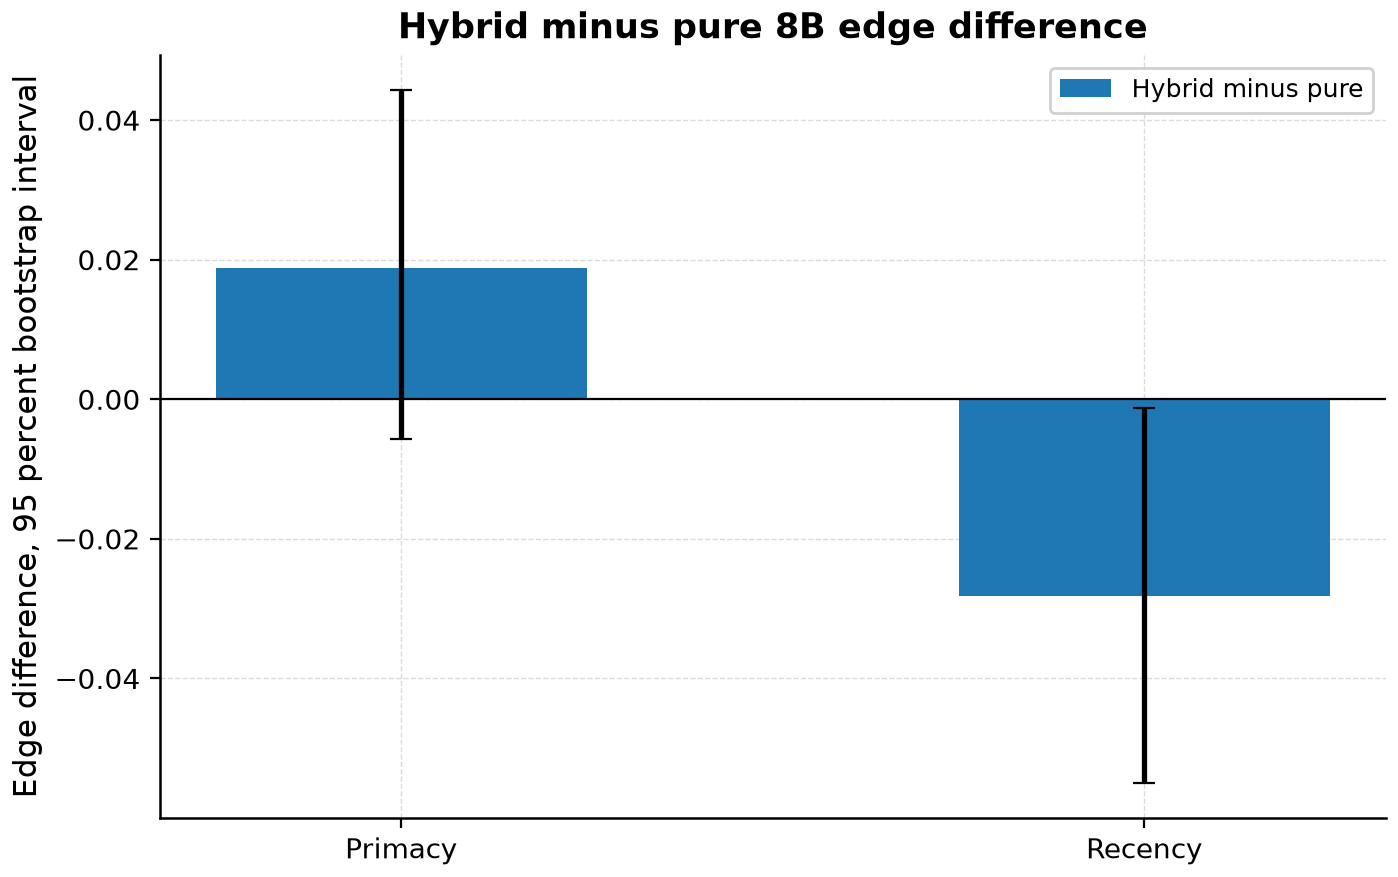
\includegraphics[width=0.44\linewidth]{figures/phase3-attention-effect.png}
\caption{Hybrid-minus-pure 8B edge effects.
The primacy interval crosses zero; recency decreases, but its Holm-corrected $p$-value is $0.089$.}
\label{fig:phase3}
\end{figure}

\section{Scope checks}
\label{sec:robust}

\paragraph{Scale.}
Across five approximate size pairs, the Pythia-minus-Mamba primacy gap is near zero at the two smallest scales and is $+0.062$, $+0.069$, and $+0.053$ in the three larger pairs (Figure~\ref{fig:phase4}).
The smallest Pythia ceiling is only $0.009$, so this is a descriptive capability-and-family trend, not evidence for a depth threshold.

\paragraph{Training corpus.}
Holding the Mamba-2.8B architecture fixed, the SlimPajama-minus-Pile primacy effect is $-0.007$ (95\% CI $[-0.030,0.016]$, $p=0.568$) and the recency effect is $-0.016$ (95\% CI $[-0.044,0.012]$, Holm $p=0.502$) \citep{soboleva2023slimpajama}.
The floor differs substantially ($0.270$ versus $0.114$), so this comparison finds no edge-shape change but does not rule out training-data effects.

\paragraph{Synthetic retrieval.}
On 50 RULER \texttt{niah\_single\_1} examples at 2K tokens \citep{hsieh2024ruler}, Pythia again has a primacy edge ($+0.12$, 95\% CI $[0.05,0.20]$).
Both Mamba models score $1.0$ at every depth, so this check reproduces the transformer pattern but cannot compare mixer curves on the synthetic task.

\paragraph{Descriptive system comparison.}
We also run \texttt{Llama-3.1-8B} \citep{dubey2024llama}, \texttt{Qwen2.5-7B} \citep{yang2024qwen2}, and \texttt{Nemotron-H-8B} \citep{nvidia2025nemotronh}.
All three show positive primacy edges ($+0.076$, $+0.041$, $+0.067$).
Only Llama versus Qwen has a significant paired primacy interaction ($+0.036$, Holm $p=0.016$).
Because the systems differ on architecture, data, tokenizer, token count, depth, and positional encoding, these results establish prevalence, not an architectural explanation.

\begin{figure}[H]
\centering
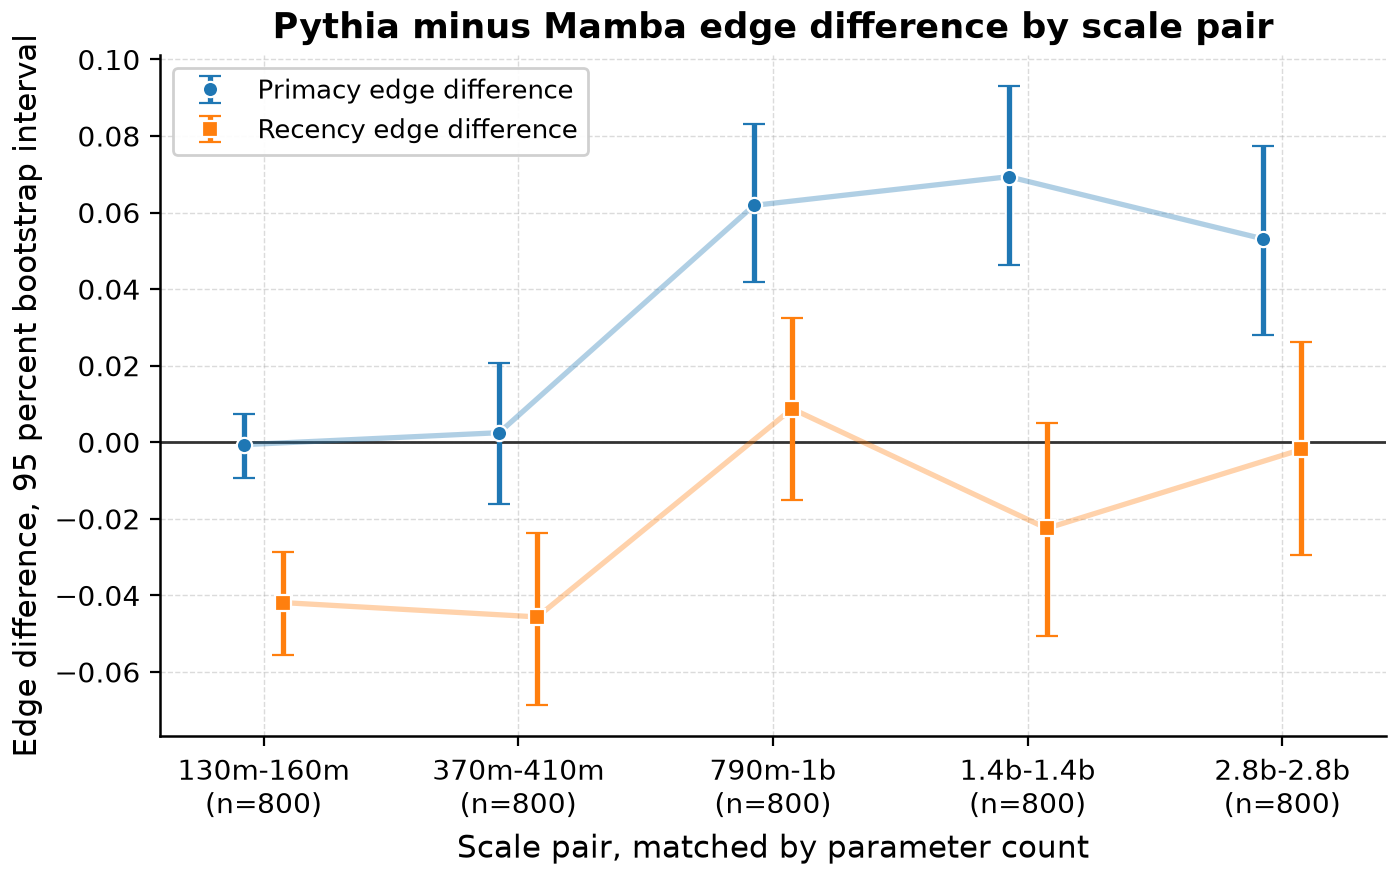
\includegraphics[width=0.46\linewidth]{figures/phase4-scale-gap.png}
\caption{Pythia-minus-Mamba edge differences across approximate size pairs.
The larger-model primacy gaps are descriptive because capability and several architectural factors vary together.}
\label{fig:phase4}
\end{figure}

\section{Mechanistic evidence and intervention}
\label{sec:mechanism}

\paragraph{Attention sinks track primacy.}
Across the Pythia family, the 160M model has almost no token-0 attention sink (final-layer share $0.003$), while the 2.8B model reaches $0.455$ \citep{xiao2024efficient}.
Pythia-410M has a small final-layer sink ($0.034$) and no significant primacy edge.
Figure~\ref{fig:sink} is consistent with a sink mechanism, but the measurements share model scale as a confound and no valid sink ablation was completed.

\paragraph{Utilization, not storage, is a hypothesis.}
A balanced linear probe on frozen mid-depth states predicts edge versus middle position above its shuffled-label control for Pythia ($0.603$ versus $0.484$) and Mamba ($0.648$ versus $0.508$).
Thus position information remains linearly decodable even when Mamba has no positive primacy edge.
This supports a utilization hypothesis, but probe decodability does not prove that the model stores or uses the answer-bearing content.

\paragraph{Training-free prompt intervention.}
On 200 exploratory questions, repeating the question both before and after the documents increases Mamba primacy from $0.000$ to $+0.103$ ($p<10^{-4}$).
Placing the question only before the documents does not create primacy ($+0.020$, $p=0.366$), but reduces recency from $+0.070$ to $+0.010$.
The intervention is training-free and practically useful, but it changes query repetition and token placement together, so it is not a clean test of fixed-state compression.

\paragraph{Prompt sensitivity.}
Changing the prompt template reduces Pythia primacy from $+0.070$ to $+0.005$ in the 200-question mechanism subset.
This result warns against treating the measured magnitude as a template-invariant architectural constant.

\begin{figure}[H]
\centering
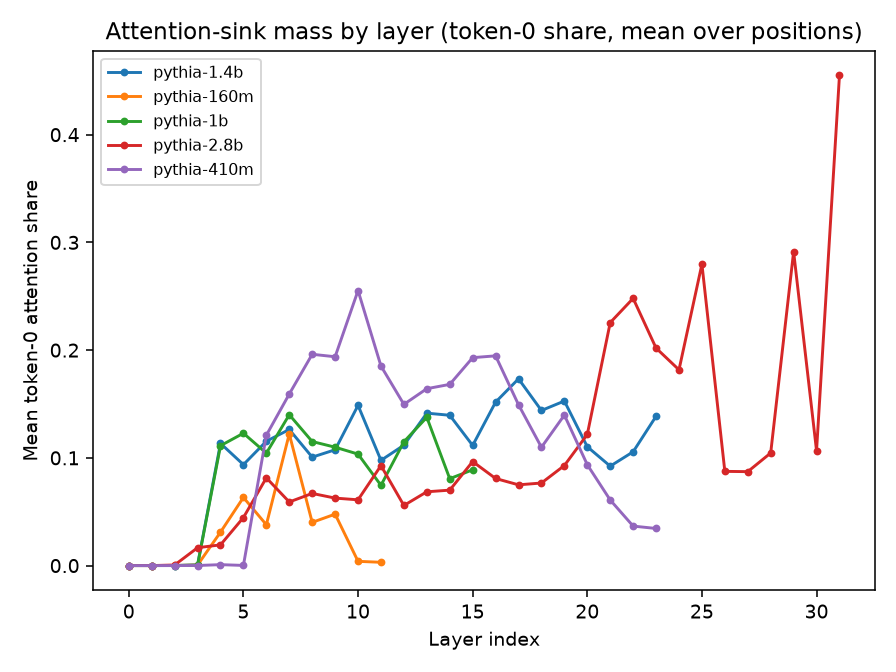
\includegraphics[width=0.45\linewidth]{figures/phase7-sink.png}
\caption{Mean token-0 attention share by Pythia layer and scale.
Late-layer sink mass covaries with primacy but is not causally identified.}
\label{fig:sink}
\end{figure}

\section{Discussion and limitations}
\label{sec:discussion}

The most secure result is the 2.8B exploratory architecture-position interaction.
The matched 8B direction, sink correlation, and probe results jointly make attention-mediated utilization a plausible hypothesis, while prompt sensitivity shows that architecture is not the only determinant.

Several limitations set the confirmatory boundary.
All analyses use the exploratory split, so the planned 1{,}855-question test must be run under a frozen analysis before confirmatory language is warranted.
The 2.8B and scale comparisons retain depth, positional-encoding, state-size, and capability confounds.
The matched 8B paired contrast crosses zero after Holm correction, and its run manifest records a dirty source tree, weakening exact reproducibility.
The negative and distractor-order controls lack committed outputs.
A 50-generation blinded audit sample exists, but human labels were not completed.
Finally, the attempted hybrid sink block did not alter the model because its custom attention path did not honor the hook; it is not an ablation result.
The next decisive study should freeze exclusions and contrasts, complete these controls, repair the hybrid intervention, and evaluate the held-out split once.

\section{Conclusion}
\label{sec:conclusion}

On 800 exploratory Lost-in-the-Middle questions, Pythia-2.8B and two Pile-trained Mamba models have different primacy profiles under a paired ten-position evaluation.
A matched 8B comparison is directionally consistent but statistically uncertain, so the present evidence supports an architecture-position interaction without establishing that attention causes it.
The held-out split and completed control suite now provide a clear path from this exploratory workshop result to a confirmatory claim.

\newpage
{
\small
\begin{thebibliography}{99}

\bibitem[An et al.(2024)]{an2024make}
C.~An, S.~Huang, J.~Zhang, et al.
\newblock Make your LLM fully utilize the context.
\newblock \emph{arXiv:2404.16811}, 2024.

\bibitem[Biderman et al.(2023)]{biderman2023pythia}
S.~Biderman, H.~Schoelkopf, Q.~Anthony, et al.
\newblock Pythia: A suite for analyzing large language models across training and scaling.
\newblock In \emph{International Conference on Machine Learning}, pages 2397-2430, 2023.

\bibitem[Dao and Gu(2024)]{dao2024mamba2}
T.~Dao and A.~Gu.
\newblock Transformers are SSMs: Generalized models and efficient algorithms through structured state space duality.
\newblock In \emph{International Conference on Machine Learning}, 2024.

\bibitem[Dubey et al.(2024)]{dubey2024llama}
A.~Dubey, A.~Jauhri, A.~Pandey, et al.
\newblock The Llama 3 herd of models.
\newblock \emph{arXiv:2407.21783}, 2024.

\bibitem[Gao et al.(2020)]{gao2020pile}
L.~Gao, S.~Biderman, S.~Black, et al.
\newblock The Pile: An 800GB dataset of diverse text for language modeling.
\newblock \emph{arXiv:2101.00027}, 2020.

\bibitem[Gu and Dao(2023)]{gu2023mamba}
A.~Gu and T.~Dao.
\newblock Mamba: Linear-time sequence modeling with selective state spaces.
\newblock \emph{arXiv:2312.00752}, 2023.

\bibitem[Hsieh et al.(2024a)]{hsieh2024found}
C.-P. Hsieh, S.~Sun, S.~Kriman, S.~Acharya, D.~Rekesh, F.~Jia, and B.~Ginsburg.
\newblock Found in the middle: Calibrating positional attention bias improves long context utilization.
\newblock In \emph{Findings of the Association for Computational Linguistics: ACL}, pages 14982-14995, 2024.

\bibitem[Hsieh et al.(2024b)]{hsieh2024ruler}
C.-P. Hsieh, S.~Sun, S.~Kriman, et al.
\newblock RULER: What's the real context size of your long-context language models?
\newblock \emph{arXiv:2404.06654}, 2024.

\bibitem[Lieber et al.(2024)]{lieber2024jamba}
O.~Lieber, B.~Lenz, H.~Bata, et al.
\newblock Jamba: A hybrid Transformer-Mamba language model.
\newblock \emph{arXiv:2403.19887}, 2024.

\bibitem[Liu et al.(2024)]{liu2024lost}
N.~F. Liu, K.~Lin, J.~Hewitt, A.~Paranjape, M.~Bevilacqua, F.~Petroni, and P.~Liang.
\newblock Lost in the middle: How language models use long contexts.
\newblock \emph{Transactions of the Association for Computational Linguistics}, 12:157-173, 2024.

\bibitem[NVIDIA(2025)]{nvidia2025nemotronh}
NVIDIA.
\newblock Nemotron-H: A family of accurate and efficient hybrid Mamba-Transformer models.
\newblock \emph{arXiv:2504.03624}, 2025.

\bibitem[Peysakhovich and Lerer(2023)]{peysakhovich2023attention}
A.~Peysakhovich and A.~Lerer.
\newblock Attention sorting combats recency bias in long context language models.
\newblock \emph{arXiv:2310.01427}, 2023.

\bibitem[Soboleva et al.(2023)]{soboleva2023slimpajama}
D.~Soboleva, F.~Al-Khateeb, R.~Myers, et al.
\newblock SlimPajama: A 627B token cleaned and deduplicated version of RedPajama.
\newblock Cerebras technical report, 2023.

\bibitem[Vaswani et al.(2017)]{vaswani2017attention}
A.~Vaswani, N.~Shazeer, N.~Parmar, et al.
\newblock Attention is all you need.
\newblock In \emph{Advances in Neural Information Processing Systems}, 2017.

\bibitem[Waleffe et al.(2024)]{waleffe2024empirical}
R.~Waleffe, W.~Byeon, D.~Riach, et al.
\newblock An empirical study of Mamba-based language models.
\newblock \emph{arXiv:2406.07887}, 2024.

\bibitem[Xiao et al.(2024)]{xiao2024efficient}
G.~Xiao, Y.~Tian, B.~Chen, S.~Han, and M.~Lewis.
\newblock Efficient streaming language models with attention sinks.
\newblock In \emph{International Conference on Learning Representations}, 2024.

\bibitem[Yang et al.(2024)]{yang2024qwen2}
A.~Yang, B.~Yang, B.~Zhang, et al.
\newblock Qwen2.5 technical report.
\newblock \emph{arXiv:2412.15115}, 2024.

\end{thebibliography}
}

\newpage
\input{checklist.tex}

\end{document}
